\chapter{Theory/Design}\label{chap:01}
\section{Scintillating Fiber Trackers}

A scintillating fiber tracker system consists of many scintillating fiber wires glued to each other side by side and in back to back layers; at the end of the fibre which a silicone photomultiplier photon measurement component is present. This component registers the actual photons created when a charged particle interacts with the scintillating fiber at any point and manages to travel down the fiber material into the silicone photomultiplier. Scintillating fibers are first combined into mats in a hexagonal order, as can be seen in \hyperref[Mats]{Figure 1.1} after which these mats are combined to cover a large enough surface area to be used in the detector as can be seen in \hyperref[Tracker System]{Figure 1.2}. In the second figure, the mirror put in between the two connected "dead" inner ends of the fibre without a measurement component can be seen. The purpose of this mirror is to reflect photons back into the fibre so the photons can reach the silicon photomultiplier end.

\begin{figure}[h]
    \centering
    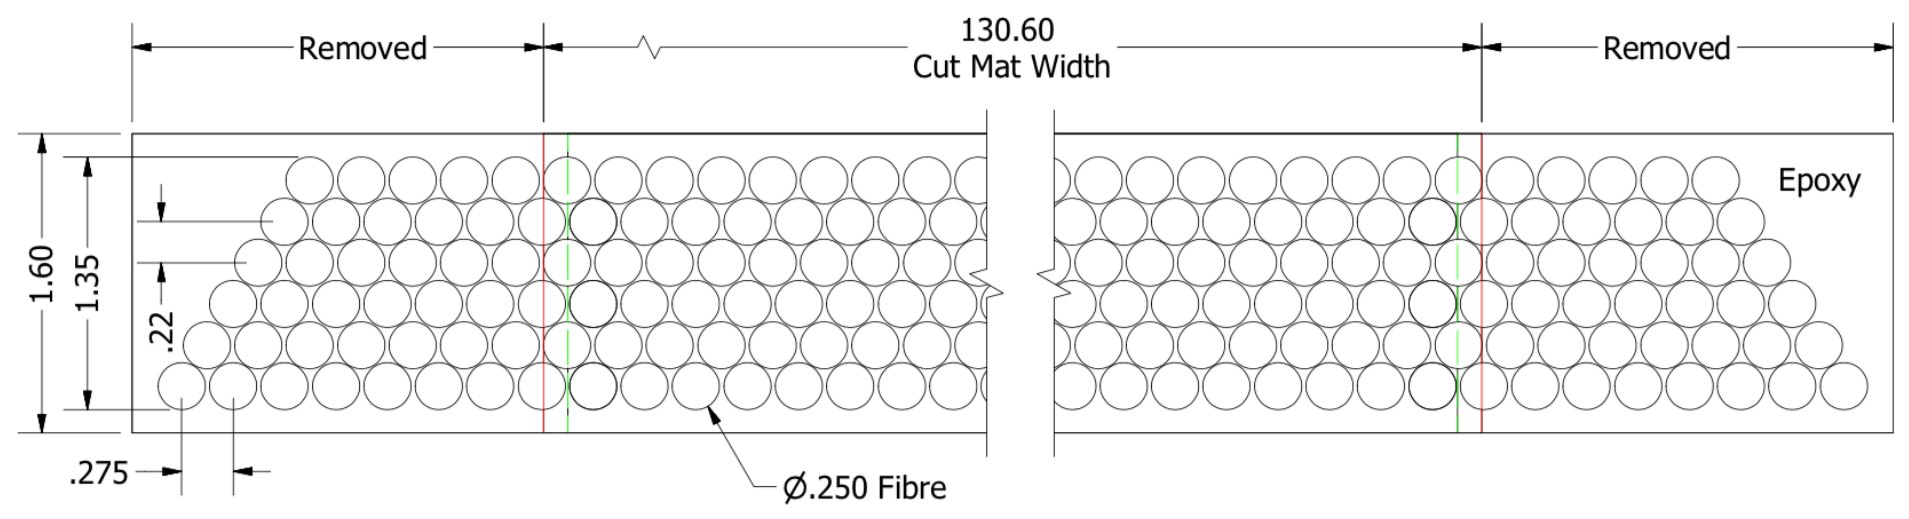
\includegraphics[width=1\linewidth]{images/SciFi Mat.png}
    \caption{Schematic cross-section of a fibre mat with six layers of fibres arrange in a hexagonal pattern. The mat is cut along the red lines.\cite{tudo}}
    \label{Mats}
\end{figure}
\newpage
\begin{figure}[h]
    \centering
    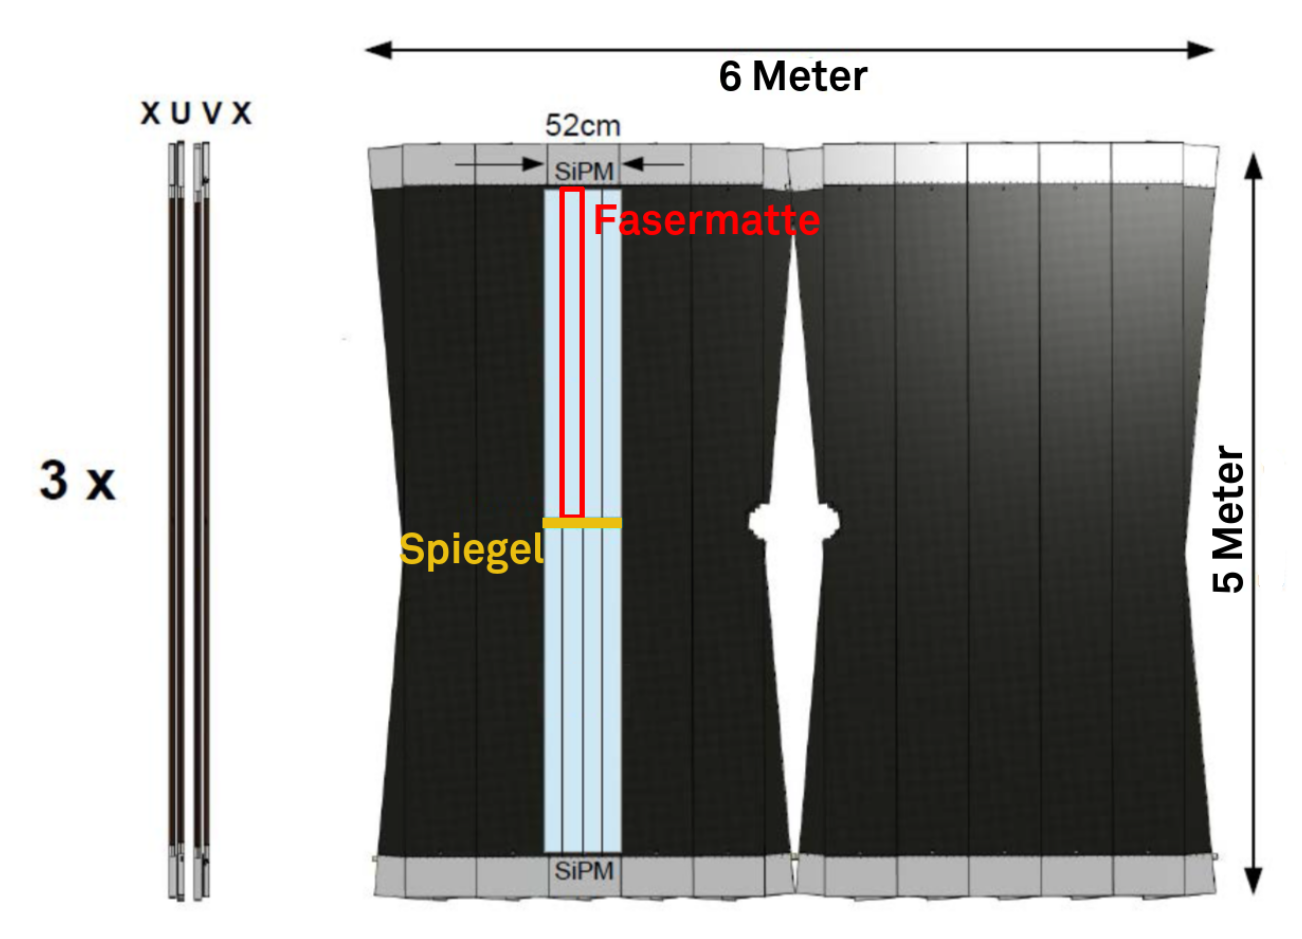
\includegraphics[width=1\linewidth]{images/SciFi tracker system.png}
    \caption{Schematic view of the SciFi Tracker. On the left side of the image is a side view of a station consisting of four layers. The right side shows a front view of the SciFi Tracker, with the two halves slightly separated. A single fibre mat is highlighted in red.\cite{tudo}}
    \label{Tracker System}
\end{figure}


The fibers in LHCb are constructed at 250 $\mu$m thickness. When a reading is measured at the photomultiplier end, the probability of the charged particle passing through a single fiber is described by a uniform distribution. The resolution of a fiber of width $d$ can be calculated using the standard deviation of a normal distribution:

$$
\sigma_{\text {fiber }}=\sqrt{\frac{d^{2}}{12}} .
$$

Inserting the LHCb scintillating fiber width of 250 $\mu$m, a resolution of $\approx 72 \mu$m is calculated. Highly penetrating particles are scattered less in the fibers compared to other trackers, consequently the systematic error introduced by the detector is kept low.

\newpage

\section{Scintillating Fiber Structure}
The fibres have an organic scintillator 220 $\mu$m thick polystyrene core, which acts as the active detector and photon propagation medium. The core is surrounded by two sheaths with outwardly decreasing refractive indices to allow an increased range of total internal reflection at the interfaces as can be seen in \hyperref[Individual Fiber]{Figure 1.3}. Each of these sheaths have a thickness of 7.5 µm, resulting in a total fiber thickness of 250 µm.

\begin{figure}[h]
    \centering
    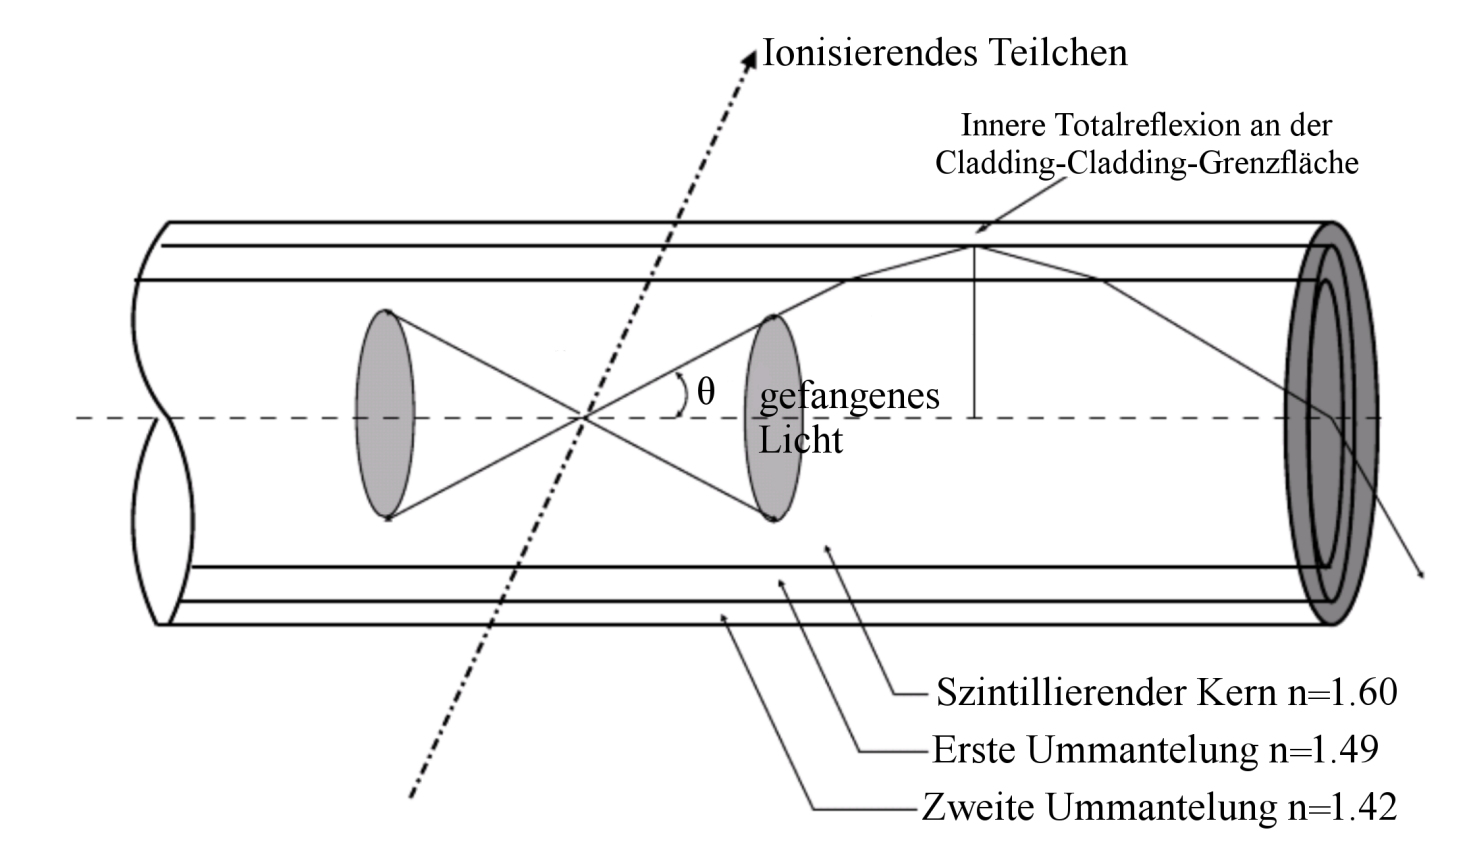
\includegraphics[width=1\linewidth]{images/Individual SciFi.png}
    \caption{Schematic structure of a scintillating fibre of type SCSF-78MJ from the company Kuraray.\cite{tudo}}
    \label{Individual Fiber}
\end{figure}

When an ionizing particle passes through and interacts with the fibre, the valence electrons of the polystyrene become excited. Excitations of electrons into higher vibrational modes transition the molecule to the $S_{10}$ energy state without radiating a photon. A photon is finally emitted when the $S_{10}$ state transitions into the ground state $S_{00}$. The difference of energy in the different energy levels in the molecule is of the order of a few eV, hence the corresponding photon is emitted in the UV range.\\

A scintillator made up of pure polystyrene is not compatible with a particle accelerator detector however, due to its long average decay time from higher energy molecule states in the order of $\approx$300 ns. In this construction, the yield in the detector is massively decreased. To combat this, the material doped with another called "p-terphenyl" which decrease the decay time to just a few nanoseconds.

\subsection{Propagation of Photon in the Fibers}
The UV photons are created in the fiber at the excitation point, which can be anywhere within the width of the core and hence have some distance from the center of the fibre. As the photon travels down the fiber, it will reflect with a certain angle $\theta$ through one of the interfaces between the core, first sheath and the second sheath or pass through the structure and get lost. The photon that is propagating in the structure will have a minimal distance $r_{min}$ from the center of the fiber as can be seen in \hyperref[Scifi Diagram]{Figure 1.4}.

\begin{figure}[h]
    \centering
    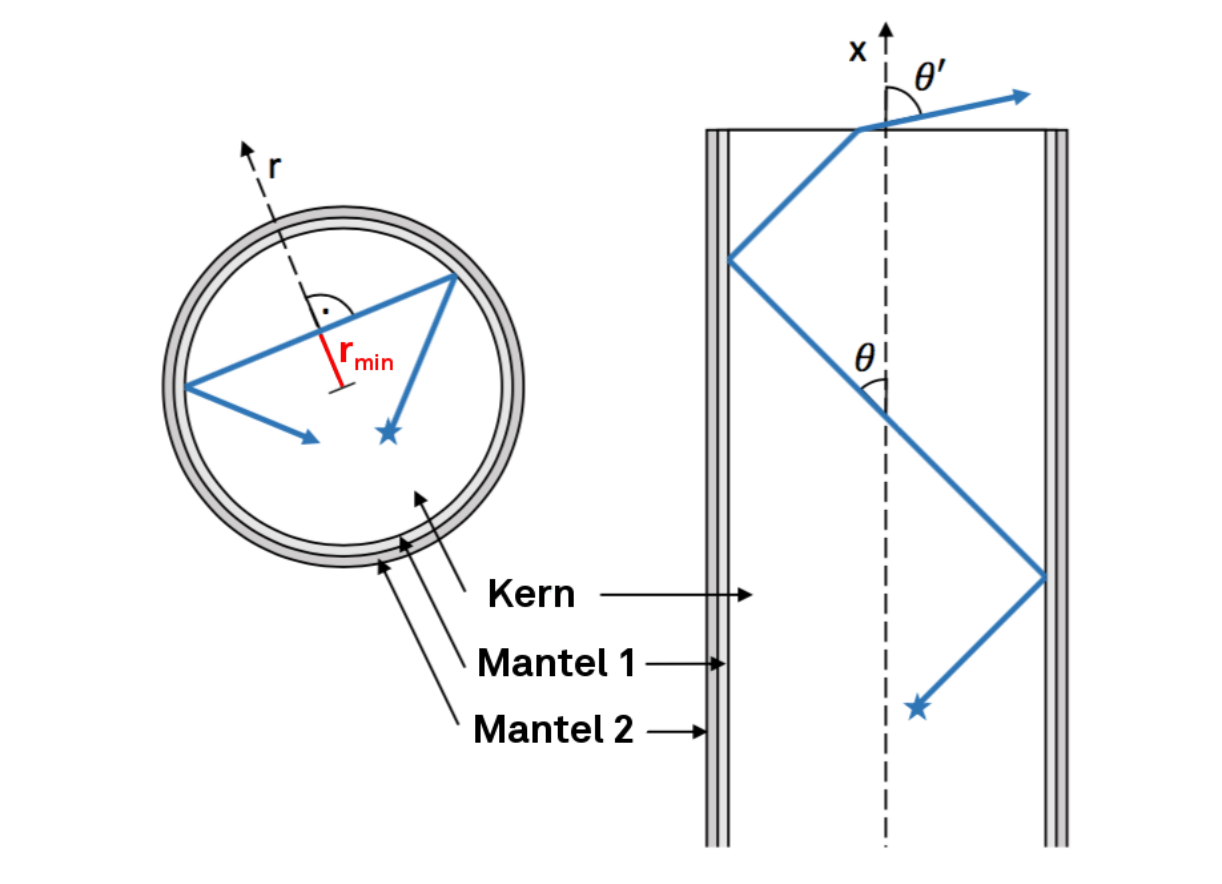
\includegraphics[width=0.8\linewidth]{images/SciFi math Diagram.png}
    \caption{Movement of a non-meridional (non-meridional: not passing through the exact center of the core) photon through the fibre. On the left side, a cross-section through the fibre is shown. The smallest distance of the photon path to the fibre axis is denoted by $r_{min}$. On the right side, a side view of the same photon path is shown. The angle $\theta$ is defined as the angle to the central axis of the fibre.\cite{tudo}}
    \label{Scifi Diagram}
\end{figure}

The length $L$ of the path a photon takes and the number of times it reflects from the interface $N$ are given by the equation:

\begin{equation}
L  =\frac{x}{\cos \theta}
\end{equation}

\begin{equation}
N  =\frac{x \tan \theta}{2 \sqrt{r_{\text {core }}^{2}-r_{\text {min }}^{2}}}
\end{equation}


Where, $r_{\text {core }}$ is the radius of the fiber core and $x$ is the distance from the end of the fiber. The reflection angle, which is the angle present at the end of the fiber $\theta^\prime_{\text {refl }}$ can be calculated using the formula:

\begin{equation}
    \theta^\prime_{\mathrm{refl}}=\arcsin \left(\sqrt{1-\frac{r_{\mathrm{min}}^{2}}{r_{\mathrm{core}}^{2}}} \sin \theta\right)
\end{equation}

The photons that are lost after creation obviously do not possess these specifications. There are many processes which contribute to lost photons such as Rayleigh scattering or absorption by the materials of the fiber. We find that there is a specific capture efficiency for all similar purpose materials that describes what fraction of photons will remain inside the fiber and make it to the end. In general, the attentuation $I$ of photons after traveling a distance $L$ in the fiber exponentially decreases according to:

\begin{equation}
\label{1.3}
I(x)=I_{0} \exp \left(-\frac{L}{\Lambda}\right)=I_{0} \exp (-a L) 
\end{equation}

Where $\Lambda$ is the attenuation length which is calculated to be approximately 3.5 meters in the specific fibers used in this experiment. The inverse attenuation length $a$ is defined as the attenuation coefficient. We can further distinguish the processes involved in the attenuation of the photon. We can express the losses due to the core material $A_{\text {core }}$ and losses due to reflection $A_{\text {refl }}$ as separate terms: 

\begin{equation}
I(x, \theta)=I_{0} A_{\text {core }}(x, \theta) A_{\text {refl }}(x, \theta)
\end{equation}

Both are exponential expression and are given as:

\begin{equation}
A_{\text {core }}(x, \theta)=\exp \left(-\frac{L(x, \theta)}{\Lambda}\right) 
\end{equation}

\begin{equation}
A_{\mathrm{refl}}(x, \theta)=\exp (-\varepsilon N(x, \theta)) 
\end{equation}

Where for reflection losses, $N$ is the number of reflections and $\varepsilon$ is the probability of loss during reflection. The final expression for the attenuation length is then obtained as:

\begin{equation}
\label{1.8}
I(x, \theta)=I_{0} \exp (-x \underbrace{\left(\frac{1}{\cos \theta}+\frac{\varepsilon \tan \theta}{2 \sqrt{r_{\mathrm{core}}^{2}-r_{\mathrm{min}}^{2}}}\right)}_{a_{\mathrm{eff}}})
\end{equation}

Here, $a_{\text {eff }}$ is defined as the effective attenuation coefficient and x is the distance from the fiber end where the excitation occurs.